\part{Proposta}
  \chapter{Como criar produtos com qualidade?}
    Quando produzimos um \textit{software}, focamos sempre nas funcionalidades que
    o sistema deve conter, pretendemos entregar o mais rápido possível e respeitar
    as datas alinhadas com o negócio. Porem, na pressa de colocar as funcionalidades
    em produção, desconsideramos os requisitos não-funcionais e por mais que a
    funcionalidade tenha sido entregue conforme o especificado, o usuário não
    consegue utilizar, consequentemente, está entrega não está gerando valor. \newline
    Como assim, os requisitos foram atendidos, mas o usuário não consegue utilizar?
    Como ignoramos os requisitos não-funcionais, o usuário pode estar sofrendo por
    diversos problemas, por exemplo, um \textit{layout} confuso, um desempenho baixo,
    o sistema está forçando ele a realizar uma tarefa que ele não está acostumado a
    fazer, ou pelo menos não no momento em que apareceu no sistema. Como entregamos
    visando a data da entrega e não o valor para o usuário, aceitamos o risco de
    entregar algo que o usuário não vê valor, e por diversas vezes cometemos erros.
    Ao testar uma funcionalidade, não costumamos ter a visão total do negócio,
    focamos na funcionalidade, então questões como tempo de resposta, ordem lógica
    no processo, localização das informações, nos passam despercebidos, não estamos
    utilizando o sistema diariamente para entender estas questões sozinhos, e o
    negócio muda frequentemente, então quando finalmente entendemos a realidade do
    usuário, ela já mudou, e voltamos a estar suscetíveis ao erro. \newline
    Como não atendemos a expectativa do usuário, e a funcionalidade não está gerando
    valor, implementamos diversas melhorias, todas o mais rápido possível, o que
    acaba gerando \textit{bugs}, como erramos uma vez, precisamos corrigir o erro
    o mais rápido possível, o que nos faz ignorar novamente requisitos não-funcionais
    e, no que lhe concerne, ignoramos questões de arquitetura de \textit{software} o que
    acaba deixando o sistema complexo, dificulta a sua manutenção, e deixa o
    sistema suscetível a erros. \newline
    Não queremos mais cometer estes erros, queremos criar o produto perfeito que
    será totalmente aderente ao usuário e que irá gerar valor para o negócio. O
    primeiro passo para gerar um produto de qualidade, que auxilia a empresa a
    concluir os seus objetivos e que traga valor ao negócio e entender que não
    existe produto perfeito. Somos humanos, erramos constantemente, realizamos
    escolhas erradas, nos equivocamos e para realizar uma entrega de pouco risco
    e extremamente assertiva, é necessário muito tempo de planejamento e de estudo,
    como, por exemplo, a construção de uma avião, ou de um prédio, ou de um equipamento
    hospitalar, estes produto não podem ter falhas, pois caso tenha, é um risco
    para a vida das pessoas e para a construção deles é utilizado muito tempo de
    planejamento, porem, nosso negócio é mais dinâmico, as necessidades mudam com
    mais frequência do que as necessidades de um avião, se utilizarmos tanto tempo
    para planejar como podemos acompanhar as mudanças do negócio?

    \section{Assumindo riscos}
      Para conseguirmos acompanhar o negócio e gerar valor para a empresa, devemos
      escolher os riscos que vamos enfrentar. Mesmo um avião encara riscos no seu
      projeto, por isso que é implementado diversas redundâncias nas funcionalidades
      mais importantes. Para identificar os riscos que vamos enfrentar e quais vamos
      conviver devemos nos perguntar, qual o objetivo do nosso projeto? Quais são
      suas funcionalidades mais importante? \newline
      Com base nisso, podemos focar a maior parte de nosso tempo no \textit{core}
      do produto, descobrindo o objetivo do sistema, alinhando com os objetivos
      da empresa, assim conseguindo prever qual será o valor para o negócio nas
      funcionalidades que iremos desenvolver. Para realizar este levantamento é
      importante considerar o nome da funcionalidade, a sua importância, os objetivos
      em que ela vai auxiliar a alcançar, os riscos que vamos enfrentar e as dependências
      para disponibilizar a funcionalidade ao usuário. \newline

      \begin{table}[h!]
        \centering
        \begin{tabular}{|c|p{10cm}|}
          \hline
          \textbf{Funcionalidade} &
          Nome da funcionalidade que será desenvolvida. \\ \hline
          \textbf{Importância} &
          A importância que a funcionalidade representa para o negócio, separada
          entre, alta, média e baixa. \\ \hline
          \textbf{Objetivos} &
          Os objetivos que a funcionalidade irá auxiliar a alcançar. \\ \hline
          \textbf{Riscos} &
          Quais os riscos que essa funcionalidade pode gerar para o negócio. \\ \hline
          \textbf{Dependências} &
          Quais são as dependências para a utilização e desenvolvimento dessa
          funcionalidade. \\ \hline
        \end{tabular}
        \caption{Definição da classificação de funcionalidades}
        \label{Tabela:1}
      \end{table}

      Toda funcionalidade deve ter um nome que represente o que será desenvolvido,
      pois, durante o desenvolvimento, é através do nome que os desenvolvedores
      vão se comunicar, sem um nome claro, que represente bem o objetivo da
      funcionalidade ao negócio e o que ela irá realizar no sistema, os desenvolvedores
      não vão conseguir se comunicar de forma clara para entender as necessidades
      do negócio. Termos e nomenclaturas devem ser estabelecidas, para que o usuário
      entenda como o sistema deve ser utilizado e para os desenvolvedores compreenderem
      como o sistema será utilizado, é através desta comunicação que a equipe de
      desenvolvimento consegue extrair os requisitos de forma fácil e formular um
      padrão de qualidade. \newline
      É necessário colocar a importância da funcionalidade que será desenvolvida, pois,
      com base nela podemos entender a ordem que vamos iniciar o desenvolvimento,
      quais riscos podemos enfrentar, definir o rigor dos testes que devemos realizar
      no desenvolvimento da funcionalidade e o padrão de qualidade para cada nível
      de importância. Embora sugerimos somente três níveis de importância (alto,
      médio e baixo), cada projeto pode criar mais níveis para classificar a
      importância da forma que a equipe se sinta mais confortável, porém, recomendamos
      não exagerar e passar de cinco, pois o principal objetivo desta classificação
      é forçar escolhermos quais funcionalidades são realmente mais importantes,
      se colocarmos muitos níveis, a funcionalidade de menor classificação será
      “alta”. \newline
      As funcionalidades que vamos desenvolver tem que estar relacionada com um
      objetivo da empresa, pois é isso que dá propósito para ela, é a nossa base
      para verificar se está gerando valor, com base no uso da funcionalidade,
      podemos verificar se o objetivo está sendo alcançado, onde com base nesse
      retorno, podemos decidir quais serão os nossos próximos passos. \newline
      Quando pensamos em uma funcionalidade, devemos sempre considerar os riscos
      para o negócio, a utilização de um sistema implica em como a operação da
      empresa trabalha, e toda mudança gera riscos para a operação. Tudo que é
      novo, deve ser ensinado, por mais que a funcionalidade reflita exatamente o
      que os usuários já faziam, eles vão começar a executar essas atividades em
      outro lugar, o que no começo pode gerar dúvidas e frustrações, devemos
      sempre levantar os riscos com base na perspectiva do usuário, pois assim
      podemos entender quais serão as reações deles e quais estratégias devemos
      utilizar para engajar o uso da ferramenta e buscar por melhorias. Com base
      nos objetivos, nas funcionalidades e nos riscos, podemos mapear as dependências
      das funcionalidades, onde conseguimos traçar quais os passos que devemos tomar
      para iniciar o desenvolvimento até disponibilizar a funcionalidade para o
      usuário. \newline
      Quando listamos tudo que estamos fazendo junto com o que o negócio pretende
      alcançar, podemos tomar decisões mais assertivas, entender dependências e
      otimizar o valor que será desenvolvido, uma vez definido nossas funcionalidades,
      sua importância e os objetivos que pretendemos com elas, podemos escolher
      quais vamos implementar primeiro e quais riscos nós vamos enfrentar. Para
      exemplificar a especificação da funcionalidade, vamos considerar uma empresa
      que possuí vendedores que entram em contato com outras empresas para negociar
      a venda de computadores. Estes computadores podem ser customizados pelo cliente,
      solicitando maior espaço de memória, se deseja um computador com \textit{SSD}
      ou \textit{HD}, qual o processador, entre outras escolhas, embora já existam
      computadores pré-montados, eles podem ser customizados somente aproveitando
      a base do produto. \newline
      Hoje a venda é feita sem a utilização de um sistema, a especificação que o
      cliente deseja é realizada de forma individual por cada vendedor e controlado
      através de planilhas, cada vendedor possui a sua forma de organizar. Somente
      o pedido final é colocado em um sistema de controle de pedidos, para emitir a
      nota fiscal. A comunicação entre os vendedores e a área técnica é feita através
      de telefone e e-mail, os produtos base e os produtos vendidos são compartilhados
      através de planilhas enviadas por e-mail, cada vendedor negocia de uma forma,
      não há padronização nas planilhas, o que acaba gerando confusões na área
      técnica na hora da montagem dos produtos. Outro ponto a destacar é que a
      área administrativa não tem visibilidade de como as negociações estão sendo
      realizadas o que dificulta o entendimento do negócio na totalidade e a criação
      de estratégias. \newline
      Com base nessas necessidades, a empresa decidiu começar um projeto para a
      criação de um sistema para os vendedores realizarem as suas negociações.
      O produto base seria disponibilizado na ferramenta e os pedidos finais
      seriam montados conforme a negociação avança, outra necessidade, é que a
      negociação deve ser faseada, para que seja possível rastrear os passos do
      vendedor e ter uma melhor visão do negócio. Após esta solicitação devemos
      levantar as principais funcionalidades para atender o negócio, colocando
      a sua importância e os objetivos que pretendemos alcançar. \newline

      \begin{table}[h!]
        \centering
        \begin{tabular}{|c|c|p{8cm}|}
          \hline
          \textbf{Funcionalidade} &
          \textbf{Importância}  &
          \textbf{Objetivos} \\ \hline
          %Funcionalidade
          Cadastro de produtos &
          %Importância
          Alta &
          %Objetivos
          Padronização na criação de produtos; \newline
          Reduzir o cadastro incorreto de produtos.
          \\ \hline
          %Funcionalidade
          Venda de produtos &
          %Importância
          Alta &
          %Objetivos
          Venda faseada do produto; \newline
          Melhor rastreabilidade da venda; \newline
          Padronização da negociação.
          \\ \hline
          %Funcionalidade
          \textit{Chat} interno &
          %Importância
          Baixa &
          %Objetivos
          Otimização da comunicação entre a área técnica e os vendedores.
          \\ \hline
        \end{tabular}
        \caption{Exemplo de levantamento de funcionalidades}
        \label{Tabela:2}
      \end{table}

      Na tabela dois, representamos três funcionalidades, o cadastro de produtos,
      a venda de produtos, e o \textit{chat} interno. Podemos notar que a maior necessidade
      da empresa é a de padronizar a venda do produto, onde a negociação deve ser
      feita de forma uniforme e que facilite os vendedores a venderem produtos
      mais aderentes com o que a área técnica consegue produzir. Com base nestas
      necessidades, foi levantado as funcionalidades de cadastro de produtos e
      venda de produtos, onde o cadastro está relacionada com a padronização da
      criação do produto e a venda está relacionada com a padronização da venda.
      Porem, a funcionalidade de \textit{chat} interno, não é uma prioridade para
      o negócio, as áreas estão se comunicando, o problema é que cada vendedor
      trabalha de um jeito, o que dificulta as decisões da área técnica. Embora um
      dos objetivos seja melhorar a comunicação entre as áreas, este não é o maior
      dos problemas que precisamos resolver, então não precisamos correr os riscos
      desta funcionalidade até o desenvolvimento das outras duas. \newline
      Outro ponto de destaque é a identificação das dependências, quando mapeamos
      elas, conseguimos ver qual funcionalidade precisamos realizar primeiro, como
      listado no exemplo, não é possível vender os produtos sem antes cadastrá-los.
      Além das dependências entre funcionalidades, podemos listar o que precisamos
      fazer para disponibilizar a funcionalidade para o usuário, como apresentado
      no exemplo, todas as funcionalidades precisam de treinamento, como o sistema
      é novo e cada vendedor realiza as negociações do seu jeito, é importante
      explicar como foi montado o processo de vendas e apresentar como realizar
      as atividades no sistema. \newline
      Cada funcionalidade tem os seus riscos, porem é através de sua importância que
      podemos criar estratégias para enfrentar estes riscos e marcar estas ações
      que definimos em nossa estratégia como dependências para liberar o uso da
      funcionalidade, desta forma os usuários não são surpresos, e é através dos
      treinamentos e das apresentações que podemos pegar o \textit{feedback} dos
      usuário e começar a mapear novas funcionalidades e melhorias. Podemos ver
      o mapeamento dos riscos e das dependências das funcionalidades criadas no
      exemplo, na tabela três. \newline

      \begin{table}[h!]
        \centering
        \begin{tabular}{|c|p{4cm}|p{6cm}|}
          \hline
          \textbf{Funcionalidade} &
          \textbf{Riscos}  &
          \textbf{Dependências}
          \\ \hline
          %Funcionalidade
          Cadastro de produtos &
          %Riscos
          Processo de cadastro de produtos mais demorado; \newline
          Criação de produtos menos flexível. &
          %Dependências
          Treinamento para cadastrar os produtos no sistema;\newline
          Explicação das regras utilizadas para o cadastro dos produtos.
          \\ \hline
          %Funcionalidade
          Venda de produtos &
          %Riscos
          Venda menos flexível; \newline
          Mudança na forma de negociação dos vendedores; &
          %Dependências
          Funcionalidade de cadastro de produtos; \newline
          Treinamento para realizar vendas no sistema; \newline
          Explicação das fases na venda.
          \\ \hline
          %Funcionalidade
          \textit{Chat} para clientes &
          %Riscos
          Não adoção do \textit{chat} como principal meio de comunicação; \newline
          Utilização do \textit{chat} para assuntos sem relação ao trabalho; &
          %Dependências
          Treinamento para a utilização do \textit{chat}; \newline
          Treinamento sobre como se comunicar por \textit{chat}.
          \\ \hline
        \end{tabular}
        \caption{Exemplo de levantamento dos riscos e dependências por funcionalidade}
        \label{Tabela:3}
      \end{table}

      \section{Entendendo os requisitos de uma funcionalidade}
        Após entendermos os ricos, escolher quais vamos aceitar e definir a prioridade
        das funcionalidades que queremos desenvolver, devemos começar a refinar cada
        uma e definir quais são seus requisitos. É importante salientar que os
        requisitos, assim como foi com os riscos, devem partir do negócio, para assim
        fazer parte do sistema, a funcionalidade deve solucionar um problema e facilitar
        a vida dos usuários, agregando valor para o cotidiano deles e consequentemente
        agregando valor para o negócio. \newline
        A funcionalidade deve ser desenvolvida com base no que os usuários já fazem
        no dia a dia, temos que mapear todas as tarefas que o usuário executa,
        identificando quais incomodam e quais não incomodam. Identificar quais tarefas
        o usuário não gosta de fazer, já é um ponto de partida de o que o sistema pode
        automatizar, uma vez que o usuário não precise fazer determinada atividade,
        já facilitou o seu cotidiano. Outro ponto de atenção, são com as tarefas que
        o usuário não se importa em executar, automatizar ou mudar a forma que ele
        trabalha, pode ser um problema em um primeiro momento, pois ele terá que
        se acostumar com essa nova forma de trabalho, embora muitas vezes essa mudança
        possa se originar em uma nova fase da empresa, que está revendo os seus processos
        e mudando a forma de trabalho dos colaboradores, é importante implementar
        a funcionalidade de forma que seja um meio-termo entre o que os usuários
        realizavam e a nova forma da empresa, desta forma os usuários começam a
        se adaptar a nova perspectiva e conforme o projeto for avançando, podemos
        ir adaptando a funcionalidade a restruturação da empresa, nenhuma mudança
        acontece do dia para a noite, uma mudança brusca na forma de trabalho
        pode gerar desconforto nos usuários e deixar eles confusos em como executar
        suas atividades. \newline
        Como o negócio está constantemente sofrendo mudanças, o sistema deve se
        adaptar para os novos requisitos do mercado, por este motivo, não devmos
        considerar os requisitos que já identificamos, como uma certeza absoluta,
        o sistema deve estar pronto para sofrer qualquer alteração e a qualquer hora.
        Dependendo de como for contruído o sistema, algumas mudanças podem levar
        muito tempo para serem realizadas, e até o seu ajuste, o requisito já sofreu
        mais uma mudança, por este motivo, devemos classificar nossos requisitos
        ao nível de importância e ao nível de mutabilidade. Enquanto nos riscos
        nós classificamos a funcionalidade na totalidade, aqui vamos classificar
        os requisitos que formam essa funcionalidade, devemos sempre analisar, o que
        é essencial para atingir o objetivo e o que pode se tornar uma melhoria para
        o futuro, desta forma, conseguimos entregar valor mais rápido para diferentes
        áreas do negócio, pois se focarmos todo o nosso tempo na funcionalidade
        mais importante, nunca vamos realizar as outras funcionalidades. Para cada
        funcionalidade devemos também atribuir um nível de mutabilidade, ou seja,
        qual é a hipótese dessa funcionalidade sofrer alterações conforme o tempo
        vai passando, embora o negócio esteja em constante mudança, sabemos que
        certos processos dificilmente sofrem alterações, pois faz parte do \textit{core}
        da empresa, é a essência do negócio. A forma de classificar a mutabilidade
        é através de porcentagem, onde as primeiras classificações serão intuições
        com base na perspectiva do negócio, mas as seguintes, conforme o sistema
        vai sofrendo alterações e melhorias, estas taxas sejam atualizadas e se
        tornem mais assertivas. Na hora de classificar é importante lembrar que
        não existe zero porcento, toda funcionalidade pode sofrer alterações,
        mesmo que demore anos para isso acontecer, a sociedade muda, novas
        tecnologias vão surgindo e o que era comum é substituído por algo novo,
        que acaba se tornando o novo comum, e se a empresa não estiver preparada
        para acompanhar essas mudanças, ela acaba se perdendo no tempo. Realizando
        essa classificação podemos identificar quais processos estão consolidados
        e quais processos ainda devem ser estruturados, com essa visão sobre os
        processos, podemos identificar o novo \textit{core} do negócio e dest
        forma trabalhar em uma transformação na empresa para atender as novas
        necessidades do mercado, assim evoluindo o sistema ou até mesmo desenvolvendo
        um novo, garantindo que a empresa se mantenha sempre atualizada com as
        tendências do mercado. Na tabela quatro estão os atributos que devem ser
        considerados quando classificamos um requisito. \newline

      \begin{table}[h!]
        \centering
        \begin{tabular}{|c|p{10cm}|}
          \hline
          \textbf{Funcionalidade} &
          Nome da funcionalidade que o requisito faz parte. \\ \hline
          \textbf{Requisito} &
          Nome do requisito que faz parte da funcionalidade. \\ \hline
          \textbf{Importância} &
          O nível de importância do requisito separado em baixo, médio e alto. \\ \hline
          \textbf{Mutabilidade} &
          O quanto este requisito pode sofrer alterações em porcentagem. \\ \hline
          \textbf{Stakeholders} &
          Quais áreas são impactadas com esta funcionalidade. \\ \hline
          \textbf{Descrição} &
          A descrição do requisito da funcionalidade. \\ \hline
        \end{tabular}
        \caption{Definição da classificação de requisitos}
        \label{Tabela:4}
      \end{table}

      Agora que temos mapeado os processos que fazem parte de determinada funcionalidade,
      e sabemos como classificar, podemos começar a levantar eles. Todo requisito
      deve possuir uma descrição, algo que instrua a equipe de desenvolvimento a entender
      o seu propósito e auxilie eles a desenvolver a funcionalidade. Quando analisamos
      um requisito, outros vão surgindo, pois, a um primeiro momento, focamos sempre
      na funcionalidade, e como o sistema deve se comportar, mas além de estruturar
      como determinada funcionalidade deve se comportar, devemos utilizar os requisitos
      para garantir a qualidade do que será desenvolvido. Através de como os
      usuários vão utilizar o sistema, podemos identificar o que precisamos
      garantir que funcione durante a utilização do usuário, questões como quantidade
      de acessos, tempo de resposta, usabilidade, métricas, devem ser requisitos
      do sistema, algo diretamente relacionado ao que vai ser desenvolvido e
      estabelecer um critério de aceitável para a utilização em produção.
      Quando especificamos os requisitos, devemos também identificar quais áreas
      da empresa será impactada pelo requisito, para os requisitos funcionais,
      devemos descrever quais são as áreas que vão utilizar esta funcionalidade,
      para os requisitos não-funcionais, identificamos as áreas que caso o requisito
      não seja atendido, serão impactadas, afetando os seus processos e podendo criar
      um bloqueio, deixando ele mais longo e impedindo certas atividades. Para
      exemplificar o levantamento dos requisitos, vamos utilizar a funcionalidade
      de “Cadastro de produtos”, utilizada no exemplo de identificação dos riscos. \newline
      Para realizar o cadastro de produtos, vamos supor que envolva três áreas, o
      \textit{marketing}, a equipe técnica e a equipe de vendas. O \textit{marketing},
      com base em suas análises de mercado e nas solicitações dos vendedores, analisam
      as tendências dos pedidos do cliente e montam projetos para novos produtos,
      este projeto é enviado para a área técnica que avalia se é viável ou não a
      sua execução, podendo aprovar ou recusar a montagem desse produto. Caso o
      produto seja recusado, a solicitação é devolvida para o \textit{marketing},
      com os motivos da recusa, onde eles podem realizar as devidas alterações ou
      cancelar o projeto. Caso aceito, a equipe técnica começa a montagem,
      realizam seus testes e validam se está aderente com o que foi proposto no
      projeto, uma vez encerrado está etapa, é anunciado aos vendedores que há um
      novo produto no catálogo e caso tenha relação à algum pedido de algum vendedor,
      ele é notificado que o produto foi produzido. \newline

      \begin{table}[h!]
        \centering
        \begin{tabular}{|c|p{10cm}|}
          \hline
          \textbf{Funcionalidade} &
          Cadastro de produtos \\ \hline
          \textbf{Requisito} &
          Notificação de projeto de produto base \\ \hline
          \textbf{Importância} &
          Média \\ \hline
          \textbf{Mutabilidade} &
          45\% \\ \hline
          \textbf{Stakeholders} &
          Área técnica \\ \hline
          \textbf{Descrição} &
          Quando um projeto de produto base for cadastrado, o sistema deve
          enviar uma notificação para a área técnica, que um novo produto
          foi cadastro e aguarda aprovação. \\ \hline
        \end{tabular}
        \caption{Exemplo de classificação de requisito funcional}
        \label{Tabela:5}
      \end{table}

      \begin{table}[h!]
        \centering
        \begin{tabular}{|c|p{10cm}|}
          \hline
          \textbf{Funcionalidade} &
          Cadastro de produtos \\ \hline
          \textbf{Requisito} &
          A notificação deve ser enviada imediatamente para a área técnica \\ \hline
          \textbf{Importância} &
          Média \\ \hline
          \textbf{Mutabilidade} &
          10\% \\ \hline
          \textbf{Stakeholders} &
          \textit{Marketing}, área técnica \\ \hline
          \textbf{Descrição} &
          A notificação da criação do projeto deve ser enviada em um intervalo de
          menos de um segundo para a área técnica. \\ \hline
        \end{tabular}
        \caption{Exemplo de classificação de requisito não-funcional}
        \label{Tabela:6}
      \end{table}

      \begin{table}[h!]
        \centering
        \begin{tabular}{|c|p{10cm}|}
          \hline
          \textbf{Funcionalidade} &
          Cadastro de produtos \\ \hline
          \textbf{Requisito} &
          O cadastro é destinado somente para produtos base \\ \hline
          \textbf{Importância} &
          Alta \\ \hline
          \textbf{Mutabilidade} &
          7\% \\ \hline
          \textbf{Stakeholders} &
          Vendas \\ \hline
          \textbf{Descrição} &
          Os produtos que serão cadastrados nesta funcionalidade deve somente ser
          produtos base, customizações serão feitas durante a venda. \\ \hline
        \end{tabular}
        \caption{Exemplo de classificação de requisito inverso}
        \label{Tabela:7}
      \end{table}

      Embora a funcionalidade de “Cadastro de produtos” tenham muitos outros requisitos,
      vamos exemplificar somente os que estão nas tabelas cinco, seis e sete.
      O requisito da tabela cinco se trata de um requisito funcional, o requisito de
      enviar a notificação para a área técnica quando um projeto for criado. Podemos
      notar que sua mutabilidade é de 45 porcento, embora o processo dificilmente possa mudar,
      a área técnica sempre deve ser informada quando um projeto for criado, pois,
      são eles que aprovam se o projeto é válido ou não porem, no futuro é possível
      que seja criada uma área somente para análise de projetos, hoje está
      concentrado dentro da mesma área que monta o produto, outra alteração é a
      adição de outra área, hoje o negócio estende que somente a área técnica deve
      ser informada porem, os vendedores também fazem parte do processo, uma vez que
      o projeto pode se tratar de uma solicitação deles, por este motivo, a área de
      vendas pode ser incluída no recebimento da requisição. Embora os vendedores
      também participem desse processo, a notificação é destinada somente para a área
      técnica, desta forma, somente esta área é \textit{stakeholder} desse
      requisito. Na tabela seis, temos um requisito não-funcional, é um requisito
      que está atrelado diretamente a qualidade da funcionalidade, ela está definindo
      que a notificação deve ser disparado com no máximo um \textit{delay} de um
      segundo da criação do produto. Para o negócio é importante que a área seja
      informada que um novo projeto foi criado imediatamente após sua criação, este
      requisito deve ser utilizado como critério de qualidade e utilizado como cenário
      de teste, não somente da criação de um projeto, mas para a criação de vários
      projetos de uma vez só. Na tabela sete, possuímos um requisito inverso, algo
      que o sistema não deve fazer, que no caso, é que a funcionalidade de “Cadastro
      de produtos” se destina somente para produtos base, ou seja, as customizações
      dos vendedores não estão incluídas nessa funcionalidade. Como a customização
      dos produtos base está sempre atrelada a venda do produto e não ao seu cadastro,
      dos tês exemplos, este é o de menor mutabilidade, pois este processo dificilmente
      será mudado e atribuir a responsabilidade ao vendedor de cadastrar um produto,
      somente por causas das customizações é uma mudança muito grande no processo
      de como é realizada a venda.

    \section{Arquitetura evolutiva}
      Após especifícarmos as nossas funcionalidades e os nossos requisitos, precisamos
      construir o nosso sistema, lembrando que conforme o produto vai evoluindo,
      mudanças deverão ser feitas para acompanhar as necessidades do negócio, para
      isso, devemos construir o nosso sistema de forma que seja fácil implementar novas
      funcionalidades e aplicar mudanças e melhorias em funcionalidades já desenvolvidas.
      Para que isso seja possível, devemos desenvolver um \textit{software} com alto
      nível de abstração, cada parte do sistema deve funcionar de forma quase
      individual, para que desta forma uma alteração realizada em alguma parte do
      sistema, não afeta as demais e assim, minimizamos \textit{bugs} e tempo de
      manutenção e desenvolvimento de melhorias. \newline
      No começo do projeto ainda não sabemos quais são as partes do sistema que
      conseguimos separar, o que deve funcionar de forma individual e o que faz
      parte desse individual. Para descobrirmos, quando desenharmos a arquitetura
      de nosso sistema, precisamos nos atentar na mutabilidade de cada requisito,
      devemos desenvolver cada funcionalidade como se ela pudesse mudar a qualquer
      hora, mas quando tivermos que tomar a decisão em qual parte deverá ficar menos
      abstraída, a mutabilidade do requisito deverá ser considerada, com base na
      mutabilidade, podemos montar o \textit{core} de nosso sistema, construir
      as funcionalidades que muito dificilmente deverão ser modificadas fazer com
      que a partir delas o sistema evolua para as outras funcionalidades, que
      dependendo do nível de mutabilidade, deverá funcionar de forma quase independente,
      desta forma, conforme o tempo for passando, podemos ir isolando as partes
      do sistema cada vez mais, a medida que a mutabilidade dos requisitos vão
      ficando mais assertivas com a realidade e novos requisitos vão surgindo, pois,
      desta forma, a equipe de desenvolvimento terá um melhor entendimento do negócio
      e conseguirá abstrair o sistema de forma mais condizente de como o negócio
      funciona. Quando obtivermos um sistema extremamente abstraído e um equipe
      de desenvolvimento com um grande entendimento do negócio, podemos evoluir
      nossa arquitetura para microsserviços, de forma que, cada parte do sistema
      é verdadeiramente um sistema apartado, com sua próprio equipe e requisitos,
      onde todas essas funcionalidades se encontram na mesma plataforma. Quando
      conseguimos evoluir nosso produto para este nível, ele deixa de ser um sistema
      para se tornar uma plataforma, um lugar onde vários sistemas vão ser executado
      para cumprir diversos Objetivos relacionados. Lembrando, que embora agora
      temos vários sistemas, realizando diversas tarefas diferentes, o objetivo
      da plataforma deve ser o mesmo de quando iniciamos o projeto, nunca devemos
      esquecer o objetivo do produto ter sido criado, porque é com base nele que
      as melhorias e os requisitos devem ser levantados, uma vez que esquecemos
      desse objetivo, nosso produto começa a realizar diversas ações que não
      estão relacionadas entre elas, sua arquitetura fica cada vez mais complexa
      e nosso produto perde seu propósito. \newline
      Uma vez que nosso produto esteja separado em vários sistemas, podemos reaproveitar
      as funcionalidades que desenvolvemos para outros produtos, e como cada sistema
      da plataforma tem a sua própria equipe, as análises realizadas no produto
      serão realizadas para cada funcionalidade , ou seja, em cada parte de valor
      do que foi desenvolvido, com esses dados, podemos analisar qual parte do negócio
      está sofrendo maior alteração, qual está gerando mais valor, qual precisa
      ser reestruturada, qual precisa de mais investimento, quais áreas podem ser
      dividas, conseguimos adquirir diversas análises realizadas pelas equipes que
      estão focadas na visão que a funcionalidade traz, cada parte da nossa plataforma
      está se preocupando com uma determinada parte do negócio e como, nossa equipe
      já conseguiu separar essas partes de uma forma que esteja completamente
      aderente a como o negócio funciona, conseguimos ter a visão de todas as atuações
      da empresa no mercado, conseguimos ter a visão do todo separado em várias
      equipes diferentes, que estão preocupadas em evoluir a sua parte e contribuir
      com as outras. Com essa visão, podemos evoluir nossos sistemas para outras
      plataformas, com objetivos diferentes, e agregando valor para o negócio de
      forma distinta. Podemos através das necessidades do mercado, e com os requisitos
      do sistema, reformular a forma que a empresa atua no mercado, identificar
      atuações secundárias da empresa, que tem potencial para se tornar primárias,
      fazer os sócios e diretores enxergarem cada pedaço que gera valor para a
      empresa e definir estratégias não tradicionais, para adquirir uma possível
      vantagem no mercado.

    \section{Estruturando o fluxo de entrega}
      Para alcançarmos nossos objetivos e desenvolvermos as nossas funcionalidades
      em tempo ágil, com qualidade e se preocupando em manter nossa arquitetura
      simples e evolutiva, precisamos estruturar o nosso fluxo de entrega, ou seja,
      precisamos definir como será o processo de desenvolvimento, verificação de
      qualidade, homologação e subida em produção. \newline
      Para cada requisito, devemos escrever os critérios de aceite, desta forma,
      quem for testar as funcionalidades, consiga compreender o que deve verificar
      e para que os desenvolvedores, compreendam como devem desenvolver a
      funcionalidade. Desta forma, além de termos desenvolvedores e testadores
      cientes de como o sistema deve funcionar, conseguimos criar um padrão de
      qualidade, que será documentado e revisado conforme o produto for evoluindo.
      Devemos criar os critérios de aceite escritos, para mapear quais testes deverão
      ser feitos para cada funcionalidade, cada requisito vai exigir um determinado
      tipo de teste, e com os critérios de aceite conseguimos identificar os cenários
      que eles devem ser executados, pois, é nos testes que vamos simular os momentos
      mais importantes para o negócio no sistema, os momentos em que o sistema não
      pode falhar. Embora cada requisito tenha o seu próprio conjunto de testes,
      é importante padronizar que todas as novas funcionalidades tenham sempre testes
      unitários e em massa, e para melhorias ou mudanças seja sempre realizado testes
      de regressão. Os critérios de aceite devem ser escritos se baseando diretamente
      nos riscos que aceitamos quando mapeamos as funcionalidades, nossos testes,
      além de garantir que os requisitos da funcionalidade sejam cumpridos, devemos
      simular as situações que mapeamos como risco, precisamos verificar como o sistema
      vai se comportar nestes cenários, desta forma, conseguimos antes de disponibilizar
      a funcionalidade para o usuário, averiguar se realmente faz sentido correr
      o risco mapeado. Para exemplificar a escrita dos critérios de aceite, vamos
      utilizar o requisito da tabela seis. \newline

      \begin{table}[h!]
        \centering
        \begin{tabular}{|c|p{10cm}|}
          \hline
          \textbf{Funcionalidade} &
          Cadastro de produtos \\ \hline
          \textbf{Requisito} &
          A notificação deve ser enviada imediatamente para a área técnica \\ \hline
          \textbf{Critério} &
          Deve ser disparado a notificação para todos os produtos que forem criados. \\ \hline
          \textbf{Critério} &
          Na notificação deve conter o nome do produto e quando ele foi criado. \\ \hline
          \textbf{Critério} &
          A área técnica deverá identificar se uma notificação já foi lida ou não. \\ \hline
          \textbf{Critério} &
          A notificação somente deve ser marcada como lida caso o usuário da área
          técnica acesse a notificação. \\ \hline
        \end{tabular}
        \caption{Exemplo de especificação de critérios de aceite}
        \label{Tabela:8}
      \end{table}

      Na tabela oito, podemos verificar os critérios de aceite para o requisito de
      notificação da funcionalidade de “Cadastro de produtos”. Podemos notar que cada
      requisito descreve como a funcionalidade deve funcionar, assim como auxilia
      como este requisito deve ser testado, deve ser testado de forma massiva,
      um dos critérios é de que cada produto deve disparar obrigatoriamente uma
      notificação, desta forma, se eu criar nove produtos de uma vez, deve ser
      gerada uma notificação para cada um dos nove produtos. \newline

      \begin{figure}[!h]
        \centering
        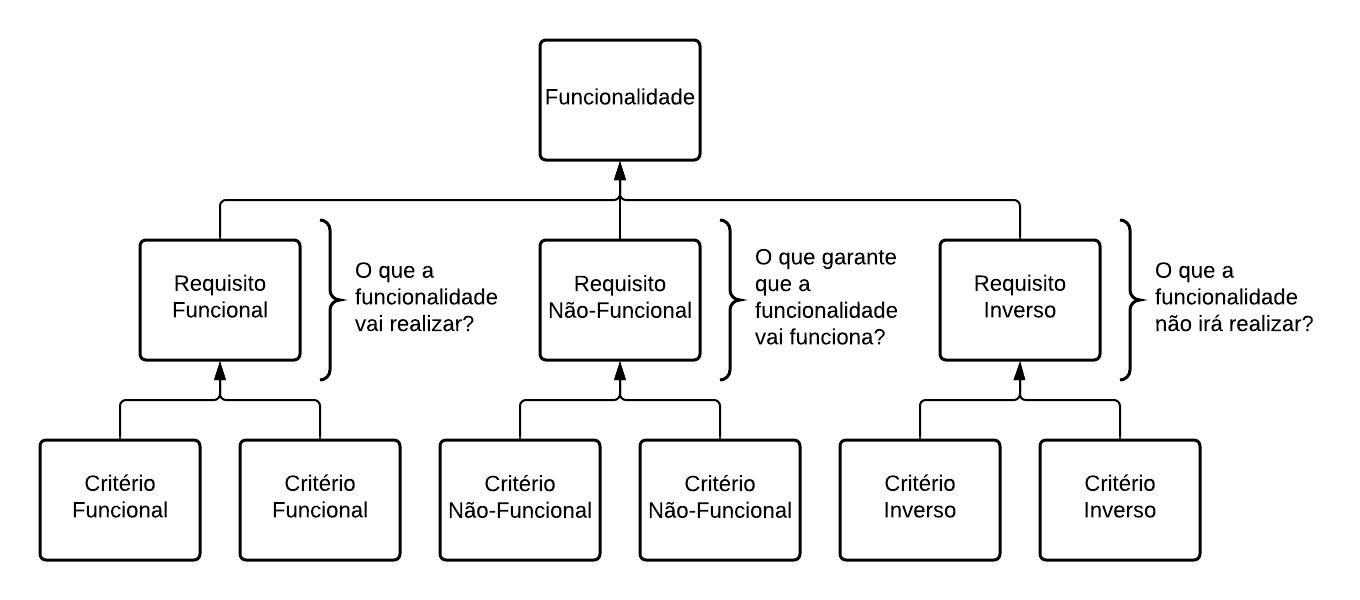
\includegraphics[width=15cm]{functionalityStructure.jpeg}
        \caption{Estrutura de funcionalidade}
        \label{Imagem:1}
      \end{figure}

      Agora que definimos como nosso requisito será desenvolvido e como ele será
      testado, precisamos definir em qual momento cada uma dessas ações deverá ser
      realizada e em qual ambiente. Quando estamos desenvolvendo uma funcionalidade
      devemos sempre testar ela por completo, mas para sermos ágeis, não podemos
      esperar todos os requisitos serem desenvolvidos para iniciarmos os testes,
      da mesma forma que os desenvolvedores não podem ficar aguardando todos os
      testes serem realizados para iniciarem um novo desenvolvimento. Enquanto os
      testadores só podem iniciar um teste assim que um desenvolvedor finalizar
      uma atividade e os desenvolvedores não podem alterar a funcionalidade para não
      influenciar nos testes, é interessante realizar estas ações em ambientes
      separados. Os desenvolvedores realizam os seus desenvolvimentos em um ambiente
      exclusivo para desenvolvimento, enquanto os testadores realizam seus testes
      em um ambiente exclusivo para testes, cada critério, cada cenário, deverá ser
      simulado neste ambiente, devido a isso a qualidade dos dados deste ambiente
      deverá ser o mais fiel possível ao que os usuários irão utilizar, por outro
      lado, os desenvolvedores necessitam de dados somente para verificar se a
      funcionalidade está funcionando e os critérios foram atendidos, devido a isso,
      é importante ter uma boa qualidade nos dados no ambiente dos desenvolvedores,
      mas não tanto quanto no ambiente dos testadores. Vamos chamar o ambiente dos
      desenvolvedores de \textbf{DEV} (desenvolvimento) e o ambiente dos testadores
      de \textbf{QA} (\textit{Quality Assurance}). \newline
      Os desenvolvedores têm a obrigação de garantir que todos os critérios do
      requisito desenvolvido sejam atendidos, ou seja, só é permitido disponibilizar
      o requisito para ser testado no ambiente de \textbf{QA} após o desenvolvedor
      testar todos os critérios no ambiente de \textbf{DEV}. O requisito disponibilizado
      em \textbf{QA}, o testador deverá testar todos os critérios nos mais diversos
      cenários possíveis, dando foco nos riscos que foram mapeados na especificação
      do requisito e conforme mais requisitos vão sendo disponibilizados, ele deverá
      testar novamente todos os cenários do requisito anterior. Desta forma, conseguimos
      garantir que as situações de maior necessidade do negócio está sendo contemplada.
      e a funcionaliadade está funcionando completamente. Para que possamos gerar
      valor de forma ágil, é importante que na primeira iteração da equipe, seja
      desenvolvida somente as funcionalidades de maior importância, pois dessa
      forma conseguimos entregar uma funcionalidade de forma rápida, embora ela
      realizando o mínimo planejado, já podemos verificar a reação dos usuários e
      identificar se há a necessidade de mudanças ou melhorias para serem desenvolvidas
      nas próximas iterações, além de reavaliar a importância dos requisitos mapeados.
      \newline
      Logo após todos os testes de todos os cenários de risco da funcionalidade
      serem executados, podemos disponibilizar a funcionalidade para homologação,
      ou seja, devemos realizar atividades com os usuário, com o objetivo de verificar
      se o que foi desenvolvido está aderente com o negócio, podemos realizar
      apresentações para os usuários, de modo a adiantar para eles o que será
      entregue e preparar uma documentação de como determinada funcionalidade
      funciona, com o intuito de disponibilizar esta informação para os usuários e
      para novos integrantes do projeto. Todo esse processo deve ser realizado em
      um ambiente separado que vamos nomear de \textbf{HOMOL} (homologação).
      Este ambiente deve estar separado, pois, os dados que contem nele,
      devem ser preparados para apresentações, como ele será utilizado para
      compreender o que será entregue e para apresentar uma prévia para os usuários,
      os cenários não devem ser influenciados por funcionalidades em desenvolvimento
      ou por testes realizados pelos testadores. Os dados neste ambiente deve ser
      o mais próximo possível do que os usuários irão utilizar em produção, as
      funcionalidades que estão neste ambiente devem estar completamente testadas
      e com todos os critérios garantidos. \newline
      Após realizarmos a homologação da nossa funcionalidade, devemos nos preparar
      para entregar ela aos usuários, para isso, vamos realizarmos uma última validação
      em um ambiente que vamos nomear de \textbf{PREPROD} (pré-produção). Este
      ambiente deve ser uma cópia perfeita de produção, nele devemos realizar novamente
      todos os principais testes que já realizamos em \textbf{QA}, para verificar
      que todos os critérios continuam sendo cumpridos, além de aplicarmos treinamentos
      para os usuários da nova funcionalidade, permitindo que eles utilizem esta
      funcionalidade de forma controlada, para que eles aprendam a utilizar o
      sistema antes de colocar em produção. Com essa abordagem, antes da funcionalidade
      ir para produção, conseguimos verificar a reação deles com o que será entregue,
      e obter uma prévia de como o sistema será utilizado, desta forma já conseguimos
      identificar melhorias para as próximas iterações. \newline

      \begin{figure}[!h]
        \centering
        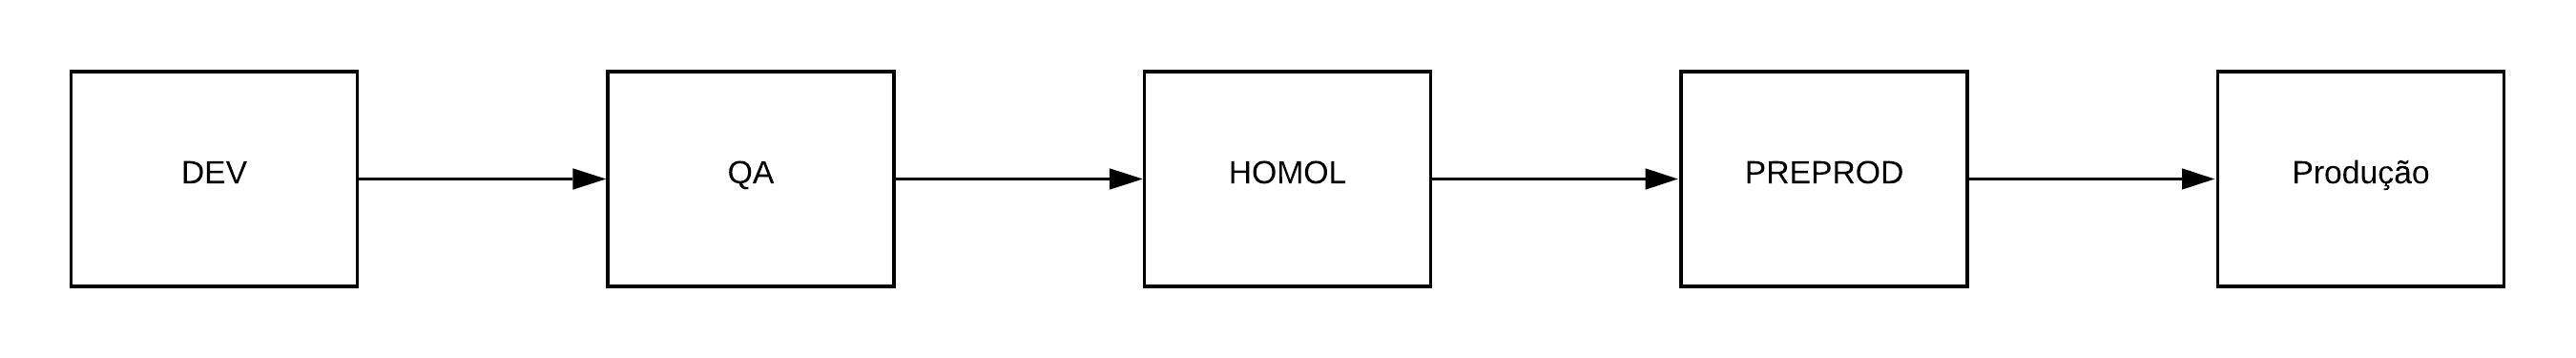
\includegraphics[width=15cm]{enviromentStream.jpeg}
        \caption{Fluxo de ambientes}
        \label{Imagem:2}
      \end{figure}

    \section{Automatizando testes de qualidade}
      Para otimizar a execução dos testes, e facilitar o trabalho dos testadores,
      podemos automatizar os testes que realizamos no sistema, para que sempre que
      uma funcionalidade nova, uma melhoria, uma alteração ou uma correção for
      implementada realizar novamente todos os testes no sistema automaticamente.
      Desta forma, não consumimos tanto tempo dos testadores e garantimos que o
      nosso sistema continua funcionando da forma que esperamos. A fase de automação
      dos testes, é importante ser realizada assim que o requisito for homologado,
      com a homologação, estamos mais certos que o requisito está aderente com o
      negócio e por causa da etapa de testes, temos todos os principais cenários
      que precisam ser garantidos, desta forma podemos montar testes automatizados
      para que após o requisito for homologado, qualquer alteração que seja realizada
      nos ambientes de \textbf{QA} e adiante, inicie os testes e garanta que os
      cenários de risco continuem não apresentando problemas para o sistema. \newline
      Os testes devem estar diretamente vinculados com o \textit{deploy} para os
      ambientes, ou seja, é importante que seja um processo do \textit{pipeline},
      onde todo \textit{deploy} realizado, rode novamente os testes para o ambiente
      que estamos levando as configurações, desta forma, conseguimos averiguar se
      alguma alteração no sistema impactou em alguma parte que não estávamos prevendo,
      possibilita encontrarmos erros antes que seja implementado em produção e
      com base nos impactos que a alteração gerou, podemos identificar o nível de
      abstração das funcionalidades e suas dependências.

  \chapter{Como adquirir escalabilidade?}
    Conforme o nosso sistema vai aumentando, mais usuários vão utilizando ele,
    mais funcionalidades ele possui, e mais poder computacional ele necessita.
    Garantir que um sistema se mantenha no ar é uma tarefa complicada, embora
    estejamos realizando testes na maioria dos cenários e evoluindo a arquitetura
    para se adequar a atual realidade do sistema, não conseguimos prever tudo, e
    muitas vezes, quando mais precisamos que ele funcione, ele apresenta algum
    problema. Podemos subestimar alguma situação ou superestimar outra, e se não
    estivermos preparados para os imprevistos, a qualidade de nosso produto pode
    cair e a confiança dos nossos usuários diminuírem. \newline
    Vamos imaginar, que a empresa que utilizamos como exemplo anteriormente,
    conseguiu criar um computador base, que atendem muitas necessidades dos seus
    clientes, devido a isso, o número de pedidos aumentou, e a empresa teve que
    contratar mais vendedores, mais colaboradores da área técnica e a equipe de
    \textit{marketing} está com várias ideias para novos produtos. O sistema
    nessa situação vai estar constantemente executando vendas, vários projetos
    serão criados, e várias notificações deverão ser disparadas. Certo dia, a
    utilização no sistema foi tão intensa, que o sistema não enviou mais notificações
    durante dois minutos, estes dois minutos foi o suficiente para que a área
    técnica não analisasse três projetos, estes projetos que a equipe de
    \textit{marketing} tinha uma grande expectativa, o tempo passou foi gerado
    um conflito entre às duas áreas, e foi identificado este erro no sistema,
    agora o momento para a produção dos produtos base se perdeu, este conflito
    abalou às duas áreas e a confiança com o sistema pelos usuários diminuiu.

    \section{Descobrindo os limites do sistema}
      Para nos prepararmos para este tipo de situações, precisamos descobrir os
      limites do nosso sistema, precisamos tentar fazer o sistema falhar em um
      ambiente controlado, antes que ele falhe em produção quando os nossos usuários
      estiverem utilizando. Entender que nosso sistema tem limites e que ele está
      suscetível a erros é o primeiro passo para descobrirmos como podemos encontrar
      estes erros, devemos utilizar os riscos que mapeamos, e simular diversas vezes
      os cenários que levantamos em nossos requisitos não-funcionais de forma a
      serem levados ao extremo, por exemplo, caso levantamos que um determinado
      requisito deve ter um tempo de resposta de no máximo dois segundos, devemos
      forçar o processamento do nosso sistema para que o tempo de resposta supere
      dois segundos e neste cenário, rodar todos os testes novamente, desta forma nós
      conseguimos ver se o fato do requisito não ser atendido tem algum impacto nos
      critérios que levantamos e uma vez conseguido simular este cenário, podemos
      mapear os limites do sistema que levou a esta cituação, como nos esforçamos
      para forçar o sistema a funcionar no seu limite, podemos documentar esse cenário
      e analisar se devemos aumentar este limite ou se aceitamos o risco que ele
      representa. Definir limites para o sistema é definir novamente os riscos que
      pretendemos aceitar, quando estávamos especificando as nossas funcionalidades,
      os riscos que mapeamos era com a perspectiva de negócio, nosso objetivo era
      garantir que o que iria ser desenvolvido, gerasse valor e não teria impactos
      negativos para os usuários, agora devemos utilizar estes riscos, em conjunto
      com os nossos requisitos não-funcionais, para mapearmos os limites do sistema,
      desta forma estamos utilizando o negócio para aprender até onde o sistema
      deve aguentar. \newline
      Quando mapeamos os limites do sistema, é importante separarmos por funcionalidade
      e buscar valores estatísticos, por mais que realizamos testes e por mais
      cenários que simulamos, não podemos garantir que em uma situação extrema,
      o sistema vai se comportar sempre da mesma forma, estamos buscando o
      extremo, esperando que o que desenvolvemos pare de funcionar e por mais que
      tenhamos uma ideia de qual parte do sistema vai falhar, não é garantido que
      as nossas expectativas sempre se cumpram, realizando o mesmo teste mais de
      uma vez, podemos ter diversos retornos diferentes e por este motivo, devemos,
      com base na importância da funcionalidade, estipular uma quantidade de testes
      para cada situação extrema. Com base nos retornos gerados, podemos documentar
      o que aconteceu e qual foi a frequência deste ocorrido, cada caso algum dia
      pode ocorrer em produção, e caso ocorra, já temos mapeado os principais
      problemas e uma vez que produção comece a trabalhar no limite do sistema,
      já sabemos o que pode ocorrer. Para armazenarmos os testes que ocorreram,
      é importante colocar anotar a funcionalidade que testamos, o cenário que
      estava o sistema e quais foram resultados com as porcentagens. Nas tabelas
      nove e dez, exemplificamos está análise utilizando a funcionalidade,
      “Cadastro de produtos”. \newline

      \begin{table}[h!]
        \centering
        \begin{tabular}{|c|p{10cm}|}
          \hline
          \textbf{Funcionalidade} &
          Cadastro de produtos \\ \hline
          \textbf{Cenário} &
          O processamento do servidor utilizado para a funcionalidade se encontra
          com 95\% de uso. \\ \hline
          \textbf{Resultado} &
          Em 89\% do cadastro de novos projetos, a notificação demorou cerca de
          três segundos para aparecer. \\ \hline
          \textbf{Resultado} &
          Em 96\% do cadastro dos novos projetos, levou cerca de dois
          segundos para realizar a criação do projeto. \\ \hline
        \end{tabular}
        \caption{Exemplo de análise de limite de sistema — limite de processamento}
        \label{Tabela:9}
      \end{table}

      \begin{table}[h!]
        \centering
        \begin{tabular}{|c|p{10cm}|}
          \hline
          \textbf{Funcionalidade} &
          Cadastro de produtos \\ \hline
          \textbf{Cenário} &
          Realizado 500 criações de novos projetos ao mesmo tempo. \\ \hline
          \textbf{Resultado} &
          Em 98\% dos cadastros a conexão com o banco de dados foi perdida ao tentar
          inserir os produtos. \\ \hline
        \end{tabular}
        \caption{Exemplo de análise de limite de sistema — limite de requisições}
        \label{Tabela:10}
      \end{table}

      Estas análises devem ser feitas em um ambiente que seja uma cópia de produção,
      sempre que algo for entregue, deve ser automaticamente replicado para este
      ambiente, vamos chamá-lo de \textbf{CHAOSPROD} (produção caótica). Os dados
      deste ambiente devem ser uma representação dos dados que contém as estruturas
      mais complexas, neste ambiente deve ser possível simular os cenários mais
      complexos para o nosso sistema, que force as nossas funcionalidades a situações
      que consideramos difíceis de ocorrer, praticamente impossíveis. Este ambiente
      deve nos fornecer a possibilidade de testar cenários em que não estamos preparados,
      identificar riscos que não mapeamos e analisar erros que ainda não aconteceram
      em produção. \newline
      Estas análises são prevendo adversidades, imaginando situações inesperadas,
      neste ambiente devemos nos concentrar nos requisitos não-funcionais, pois,
      é através das situações que vamos simular nele que vamos conseguir avaliar
      se os limites que aceitamos em nosso sistema realmente está aderente as
      necessidades do negócio, e antes que comece a aparecer situações semelhantes as
      que simulamos neste ambiente em produção, conseguimos nos preparar e criar
      um plano para que o erro que foi gerado em \textbf{CHAOSPROD} não ocorra.
      Estas análises devem ser realizadas sempre após que um requisito for entregue
      em produção, desta forma, enquanto estamos verificando como o usuário está
      utilizando a funcionalidade em produção e estamos levantando novas métricas
      para aprender sobre como podemos melhorar o sistema, com os testes realizados
      em \textbf{CHAOSPROD}, conseguimos identificar métricas para manter o
      sistema em funcionamento e melhorar a especificação dos nossos requisitos
      não-funcionais.

      \begin{figure}[!h]
        \centering
        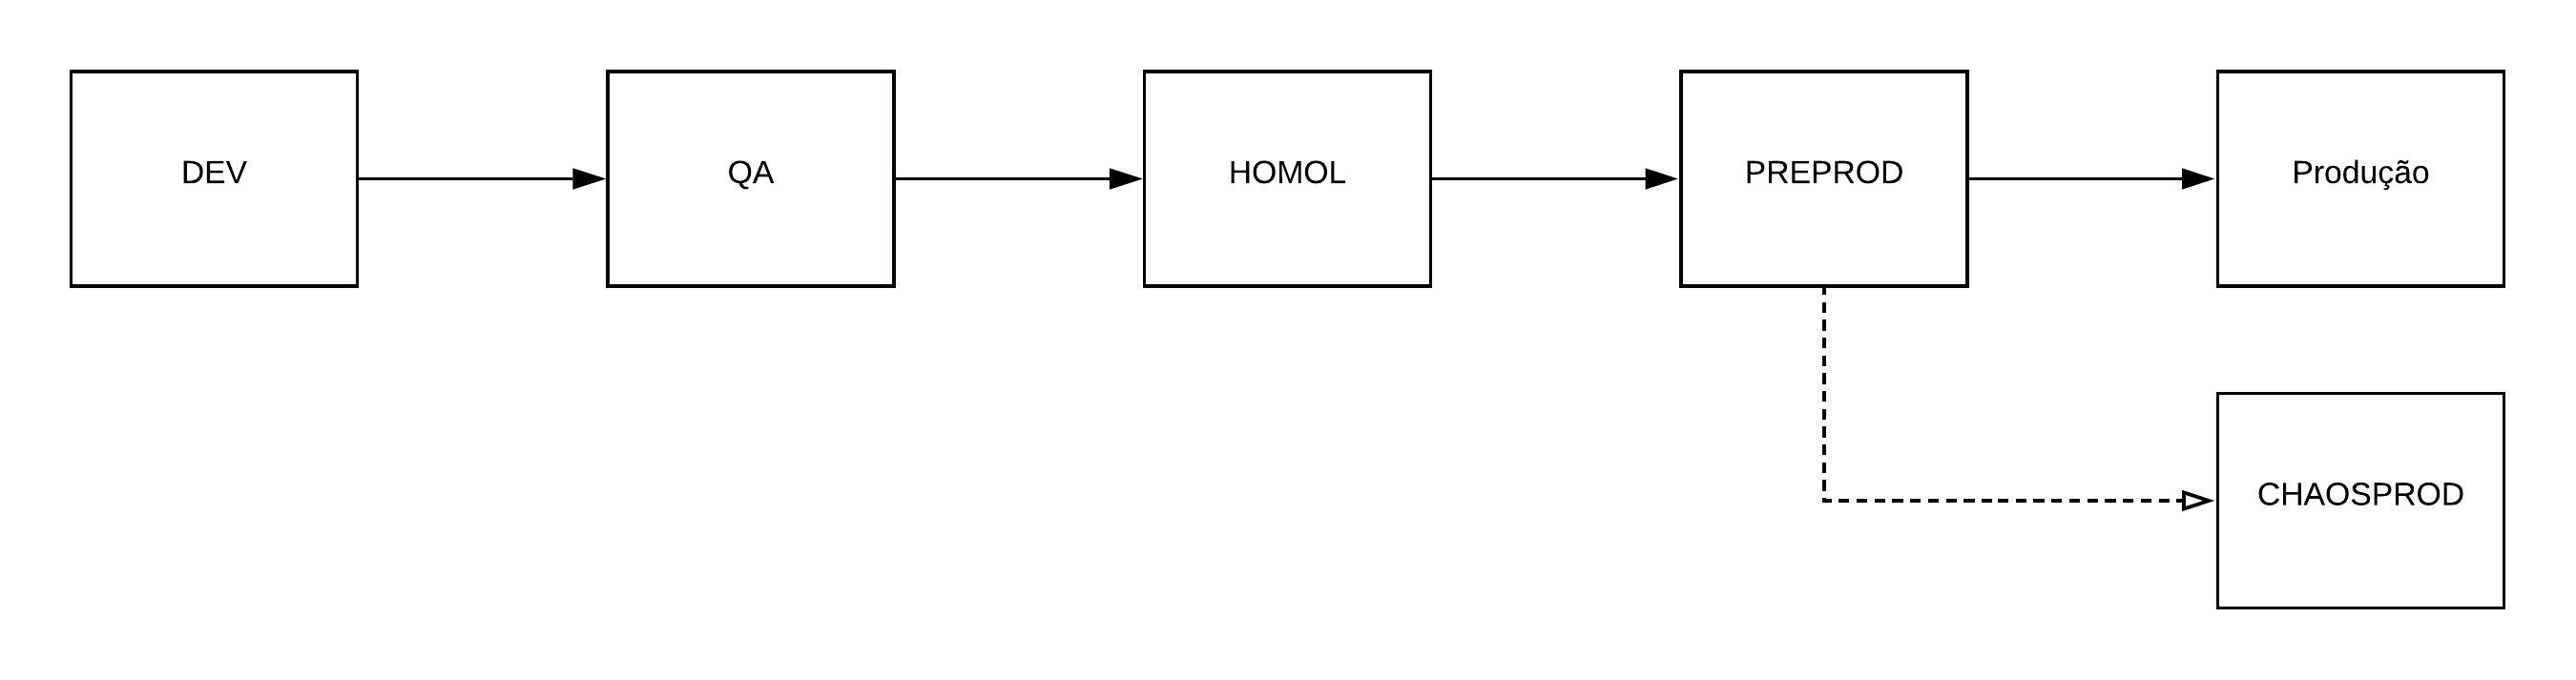
\includegraphics[width=15cm]{enviromentStream_CHAOSPROD.jpeg}
        \caption{Fluxo de ambientes com CHAOSPROD}
        \label{Imagem:3}
      \end{figure}

    \section{Desenvolvendo estratégias de escalabilidade}
      Uma vez identificado os nossos limites, devemos criar estratégias para lidar
      com elas, podendo ser aumentar o poder de processamento dos nossos servidores,
      migrar a nossa aplicação para um banco de dados mais robusto, melhorar o
      desempenho da funcionalidade desenvolvida através do código, existem
      várias ações que podemos tomar para podermos lidar com os limites mapeados.
      Para cada cenário precisamos criar um plano para caso o limite estoure. Este
      plano, deve estar atrelado diretamente a importância da funcionalidade e os
      impactos que sua execução irá gerar, devemos considerar os gastos financeiros,
      o tempo que o plano vai demorar para ser executado, as equipes que irão atuar
      nele, as áreas de negócio que vão ser impactadas e como devemos avisar os
      usuários. Com a realização deste plano, nos preparamos para o imprevisto,
      caso algum dos cenários que mapeamos aconteça, já vamos estar preparado,
      embora não sabemos exatamente o que vai acontecer, temos a probabilidade de
      cada situação. Podemos também nos antecipar a esse limite, caso a funcionalidade
      seja muito importante para o negócio, e o limite identificado possa ser atingido,
      podemos trabalhar para aumentá-lo, como sabemos aonde precisamos melhorar,
      basta realizar uma exploração mais aprofundada da melhor forma que podemos
      realizar este aumento. Outro ponto de destaque, é que conseguimos adaptar o
      nosso sistema conforme as necessidades de negócio, caso uma determinada
      funcionalidade necessite de mais processamento, podemos alocar mais servidores
      para esta funcionalidade, caso um não tenhamos os servidores disponíveis,
      podemos comprar mais servidores, caso não haja verba disponível para aumentar
      a quantidade, podemos desativar uma funcionalidade menos importante para
      realocar os recursos para a funcionalidade de maior importância, assim
      mitigamos o problema até que o período de maior necessidade passe, após esse
      período, reativamos a funcionalidade antiga e desenvolvemos um plano para
      resolver o problema. \newline
      Para cada caso devemos estruturar uma estratégia e devemos utilizar de métricas
      no ambiente de produção para supervisionar a saúde do ambiente e anteciparmos
      algum tipo de erro. Devemos monitorar o armazenamento já utilizado pelo nosso
      sistema, para o caso dele ester no fim, podemos aumentar o nível de armazenamento
      ou excluir registros antigos, devemos monitorar os nossos servidores, para
      caso algum deles estejam começando a apresentar defeito, ou algum conjunto
      de servidores estejam sendo mais utilizados que outros, assim podemos realocar
      as nossas funcionalidades em servidores diferentes e aprendemos qual parte
      do sistema utiliza maior quantidade de recursos. Podemos utilizar diversos
      acompanhamentos e implementar diversas métricas em nosso produto, mas é
      importante sempre lembrar, que devemos gerar as nossas métricas e basear a
      nossa supervisão com base em como o sistema está sendo utilizado, ou seja,
      é através das necessidades do negócio, que aprendemos aonde devemos olhar.
      Na tabela onze, especificamos como estruturar uma estratégia.\newline

      \begin{table}[h!]
        \centering
        \begin{tabular}{|c|p{10cm}|}
          \hline
          \textbf{Funcionalidades} &
          Nome das funcionalidades que foram impactadas \\ \hline
          \textbf{Cenário} &
          Descrição do cenário em que ocorreu os erros. \\ \hline
          \textbf{Stakeholders} &
          Quais são as áreas de negócio que serão impactadas no cenário descrito. \\ \hline
          \textbf{Times} &
          Quais são os equipe relacionados para a execução deste plano. \\ \hline
          \textbf{Plano} &
          O que deverá ser feito caso produção se encontre neste cenário. \\ \hline
          \textbf{Tempo de Execução} &
          Tempo para a execução do plano. \\ \hline
        \end{tabular}
        \caption{Especificação para estruturação de estratégias}
        \label{Tabela:11}
      \end{table}

      Com o ambiente de \textbf{CHAOSPROD}, conseguimos descobrir os limites do
      sistema, com o ambiente de produção, conseguimos descobrir como o sistema é
      utilizado, através dos usuários e da percepção de valor gerado para eles
      e para o negócio que devemos basear as nossas prioridades e ajustar a
      importância das nossas funcionalidades. Com está visão podemos tomar a decisão
      aonde precisamos testar mais, e também onde precisamos de maior supervisão,
      embora estejamos constantemente procurando por erros, não estamos livres de
      falhas, erros em produção vão acontecer e é nestas horas que as ferramentas
      que implementamos para supervisionar o sistema tem sua maior utilidade, é
      através delas que vamos descobrir o que aconteceu e uma vez descoberto, vamos
      utilizar este ocorrido como aprendizado, além de resolver o problema, vamos
      identificar o porquê que ele aconteceu, se realmente resolvemos o problema ou
      mitigamos, se ele pode acontecer novamente e como podemos nos preparar para
      ele. Este erro deve se tornar mais um teste automatizado para ser realizado
      durante os desenvolvimentos ou deve se tornar mais uma análise a ser feita em
      \textbf{CHAOSPROD}. De toda forma, ele se tornou um aprendizado para o produto
      e agora faz parte de um cenário que estamos prevendo, pode ser que ele
      aconteça novamente, mas desta vez estaremos preparados. \newline
      Para evitar que os cenários que identificamos em \textbf{CHAOSPROD} aconteçam
      em produção e conseguirmos monitorar problemas que não mapeamos é importante
      monitorar se os critérios que definimos para cada requisito de cada funcionalidade
      continua assegurado, precisamos criar métricas em produção para monitorar
      o sistema e verificar se nossas funcionalidades continuam funcionando como o
      esperado, é importante destacar que precisamos verificar se a funcionalidade
      está sendo utilizada, se o tempo de resposta continua sendo o que tínhamos
      mapeado em nosso requisito não-funcional, se a atividade que o usuário está
      executando, está levando o sistema à algum limite que definimos, se este
      cenário foi testado em \textbf{CHAOSPROD}, precisamos averiguar se o
      produto continua gerando valor ou se vamos precisar implementar alguma
      melhoria. Para realizar está análise, precisamos voltar para as funcionalidade
      e rever tudo o que havíamos definidos para elas, voltando para a fase de
      sua escrita, desta forma, vamos rever sua importância, os objetivos que ela
      está atrelada e consequentemente identificar novos requisitos e ajustar
      requisitos já existentes, modificando critérios e adicionando novos e
      assim que a funcionalidade for redefinida para as novas necessidades do
      negócio, voltamos para a fase de desenvolvimento, testes, comunicação,
      testes em \textbf{CHAOSPROD} e criamos métricas para garantir que
      os critérios continuem garantidos.

      \begin{figure}[!h]
        \centering
        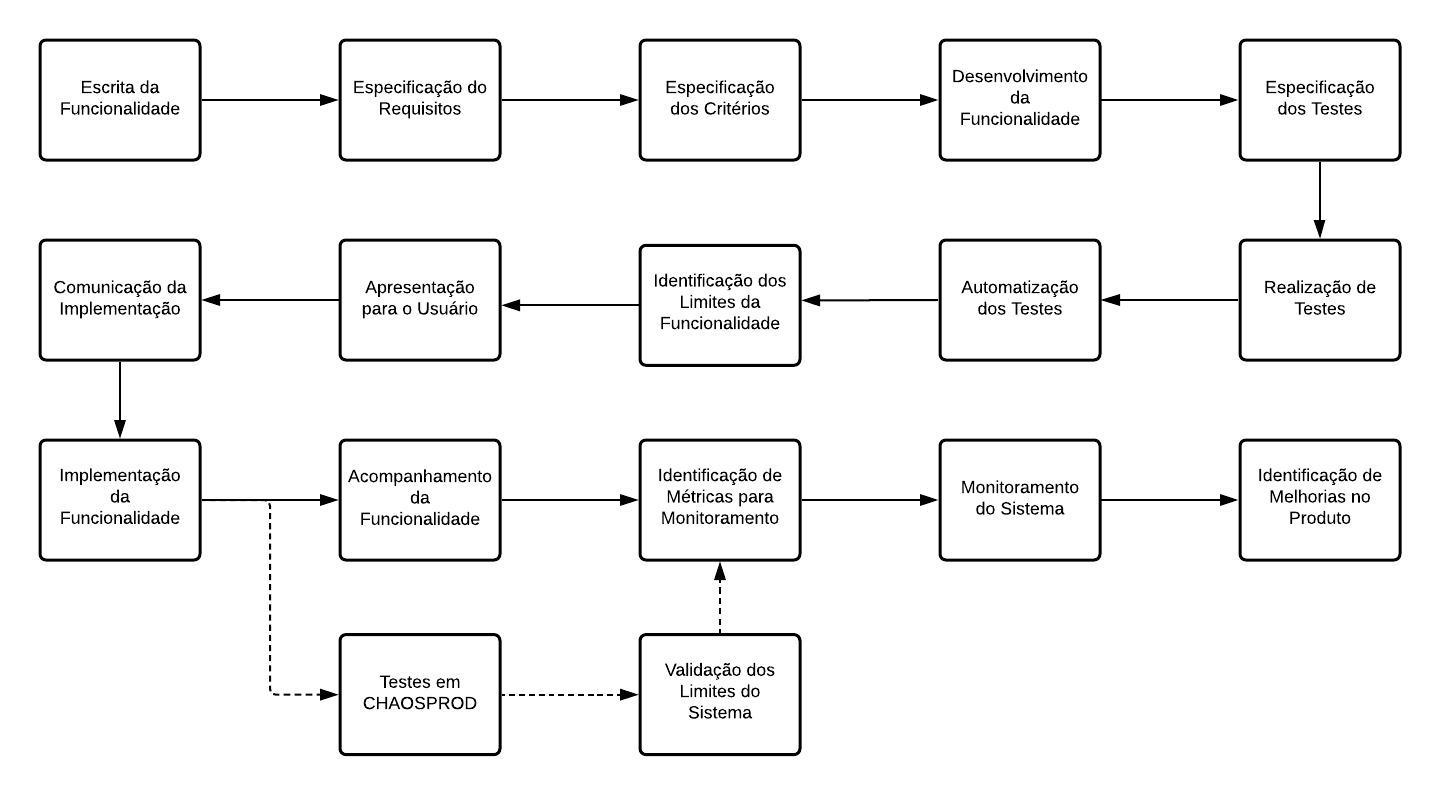
\includegraphics[width=15cm]{deliveryStream.jpeg}
        \caption{Fluxo de entrega}
        \label{Imagem:4}
      \end{figure}

  \chapter{Como manter o seu produto?}
    Para assegurar que o produto continue disponível, gerando valor, seja confiável
    para o usuário e que continue evoluindo com o negócio, nós precisamos enxergar
    a saúde do produto, isso não quer dizer apenas analisar questões do sistema
    como, desempenho, \textit{bugs}, quantidade de armazenamento e entre outros.
    Nós precisamos visualizar como o sistema está impactando o negócio, qual o
    valor que ele está produzindo e qual a percepção do usuário durante a sua
    utilização, precisamos além de captar se o sistema ainda está funcionando,
    precisamos de um ponto de vista operacional, temos que verificar se ele ainda
    está funcionando para o negócio, temos que garantir todo dia que ele seja um
    facilitador para os usuários e não um problema, precisamos sempre verificar
    se o sistema está indo de encontro com os objetivos do negócio. \newline
    Para conseguirmos estes insumos, precisamos primeiramente garantir a confiança
    do usuário, eles precisam estar seguros nas ações que eles vão realizar no
    sistema e caso uma melhoria mude a forma que eles realizam as suas atividades,
    é importante informar os usuários o motivo desta alteração e apresentar o
    objetivo da empresa com a mudança do processo. Um usuário informado, com
    confiança que o sistema funciona e que atende as necessidades dele, se torna
    um colaborador para o produto, é através do \textit{feedback} dele que conseguimos
    identificar melhorias que devemos realizar e como realizar as comunicações de
    novas implementações. Com base no como o usuário está utilizando o sistema
    é que conseguimos melhorar os nossos testes automatizados e garantir cada vez
    mais qualidade para o nosso produto, o negócio está sempre em constante
    mudança, então precisamos sempre adaptar as nossas funcionalidades para essas
    mudanças. Através dessas mudanças, novos requisitos vão surgindo, novos
    limites serão encontrados e novos riscos irão surgir, com isso mais escolhas
    e mais testes serão necessários para garantir que o sistema continue disponível
    e aderente ao negócio.

    \section{Ouvindo os usuários}
      Há diversas ações que podemos realizar para conseguirmos captar as percepções
      do usuário. A primeira delas é perguntar diretamente para eles, utilizar
      a opinião de cada usuário para tentar identificar as suas opiniões, buscando
      entender se o produto está aderente ao negócio, melhorias que devem ser
      implementadas e novas funcionalidades que devem ser desenvolvidas,
      lembrando de classificar a importância de cada nova funcionalidade ou de
      cada novo requisito. Nestas perguntas é essencial que seja identificado também
      questões de usabilidade do que já foi desenvolvido, identificar se as
      operações que eles realizam estão com um bom tempo de resposta, se o
      \textit{layout} não está confuso, se a forma que eles estão interagindo com
      as funcionalidades faz sentido para eles, se houve algum \textit{bug} ou
      situação que não funcionou como o esperado. Através destas perspectivas é
      que conseguimos garantir que os usuários estão satisfeitos ao utilizar o
      sistema. \newline
      Outra ação que devemos realizar para verificar a interação do usuário com o
      sistema, é criar métricas que informe como ele está sendo utilizado. Podemos
      medir o tempo que um usuário leva para realizar uma atividade, para verificar
      se determinada operação está com um bom desempenho, podemos medir a quantidade de
      cliques em tela, para verificar se o usuário precisa realizar muitas atividades
      para concluir o seu objetivo, campos em um formulário, para identificar se
      todas as informações ainda fazem sentido o usuário preencher, automatizamdo
      o preenchimento de alguns campos, ou até mesmo removendo eles. Para cada
      funcionalidade devemos elaborar quais métricas produzir para conseguir
      supervisionar a interação do usuário com o sistema e identificar um \textit{bug}
      durante a utilização do usuário antes mesmo que ele reporte o problema para
      o suporte. Outra análise que podemos fazer com esses dados é a de verificar
      se determinada funcionalidade está apresentando sinais de defeito, podemos
      averiguar, por exemplo, que determinada funcionalidade nos últimos três dias,
      está apresentando maior lentidão em sua execução, com essa informação podemos
      investigar se esta ocorrendo devido a alguma implementação recente, se um
      servidor está apresentando defeito, se os usuários estão realizando mais
      requisições para está funcionalidade, se a distribuição de processamento nos
      servidores está aderente a utilização dos usuários para cada funcionalidade,
      entre outras análises. Notamos que somente este dado, nos abriu diversos pontos
      de análise, que combinados com outras métricas, podemos encontrar a origem
      do problema, antes mesmo que o usuário perceba, conseguindo assegurar que
      o sistema se mantenha disponível e manter a confiança do usuário no produto.

    \section{Aprendendo com os erros}
      Com o frequente acompanhamento das funcionalidades, vamos identificar
      diversos erros cometidos no produto, o fato de estarmos monitoramento o nosso
      produto e de desenvolvermos as funcionalidades centrado no negócio, é o que
      vai nos fazer perceber os nossos erros rápido, e também vai auxiliar
      a encontrar a solução de forma rápida. Uma equipe que entende o negócio,
      sabe os requisitos de cada funcionalidade, sabe os riscos que aceitamos,
      conhece os limites do sistema e consegue monitorar a saúde do produto, tem
      completa capacidade de resolver os problemas e aprender com eles. \newline
      Quando nos deparamos com algum problema em produção, devemos analisar ele
      imediatamente, envolvendo todas as pessoas da equipe que tem ralação com o
      acontecido, seja porque trabalhou na funcionalidade ou as métricas apontam
      que é necessário a participação de um equipe especifica, como, por exemplo, a
      equipe de infraestrutura, é necessário juntar todos os envolvidos para que
      possamos realizar a análise de forma conjunta e identificar a tratativa de
      uma forma ágil. No momento da análise, é importante lembrar que não há
      culpados, devemos focar na solução do problema, depois de solucionado, é
      importante documentar o ocorrido com a solução que foi realizada e a origem
      do problema. Quando aprendemos com os nossos erros e não repreendemos a
      equipe conseguimos garantir que qualquer problema que ocorra, os membros do
      nossa equipe não vão sentir medo de reportar e todos vão trabalhar em conjunto
      para resolver o ocorrido. Após resolvido o problema, devemos mapear o que
      podemos desenvolver para supervisionar o sistema, com o objetivo de identificar
      sinais que o erro vai voltar a ocorrer e que facilite a nossa análise para
      a sua resolução. \newline

      \begin{table}[h!]
        \centering
        \begin{tabular}{|c|p{10cm}|}
          \hline
          \textbf{Funcionalidades} &
          Nome das funcionalidades que foram impactadas. \\ \hline
          \textbf{Cenário} &
          Descrição do cenário em que ocorreu os erros. \\ \hline
          \textbf{Stakeholders} &
          Quais são as áreas de negócio que foram impactadas no cenário descrito. \\ \hline
          \textbf{Problema} &
          Descrição do problema que ocorreu. \\ \hline
          \textbf{Origem do Problema} &
          O que foi que causou o problema descrito. \\ \hline
          \textbf{Equipes Envolvidas} &
          Quais equipes foram envolvidas para a resolução. \\ \hline
          \textbf{Solução} &
          O que foi realizado para resolver o problema. \\ \hline
          \textbf{Novos Desenvolvimentos} &
          O que deve ser desenvolvido para monitorar o cenário descrito com o
          objetivo de nos alertar ou facilitar a análise caso o erro volte a
          acontecer. \\ \hline
        \end{tabular}
        \caption{Especificação para documentação de resolução de problemas}
        \label{Tabela:12}
      \end{table}

      Vale lembrar que um erro, não é somente um mau funcionamento de alguma
      funcionalidade, mas sim qualquer impacto negativo para o negócio. Uma
      funcionalidade que não esteja aderente com as necessidades do usuário, deve
      ser tratada como erro, todos os envolvidos devem se reunir e discutir o que
      deve ser feito para atender as necessidades do usuário. Muitas vezes neste
      caso, os requisitos irão sofrer alterações e teremos que refazer alguma parte
      da funcionalidade, esta alteração deverá gerar novos testes automatizados
      e a arquitetura construída terá que se adaptar a estas mudanças, podendo ter
      que mudar um componente inteiro para garantir a aderência ao negócio.

    \section{Testes automatizados como ferramenta de aprendizado}
      Conforme vamos realizando mudanças no produto, seja proveniente de algum erro,
      por mudanças no negócio ou na implementação de alguma melhoria, devemos produzir
      novos testes automatizados para garantir que os novos requisitos dessas mudanças
      estejam sendo testados e garantidos. \newline
      Além de garantir a qualidade do produto, os testes têm a função de servir
      como base de conhecimento, é a partir deles que podemos analisar todos os
      processos que desenvolvemos para o negócio e explicar o funcionamento das
      funcionalidades. Nos testes automatizados simulamos como o usuário vai
      interagir com o sistema, verificamos se todos os tipos requisitos estão
      sendo garantidos, funcionais, não-funcionais, inversos, conseguimos demonstrar
      tudo o que foi feito para garantir a qualidade das funcionalidades assim
      como descrevemos o seu funcionamento, desta forma, conseguimos utilizar os
      testes automatizados, como documentação do produto como todo, seja para um
      novo membro da equipe ou para um novo usuário, podemos demonstrar o funcionamento
      de uma nova funcionalidade, para os usuários envolvidos, podemos explicar
      como funciona um determinado processo da empresa, como os testes simulam
      a forma que o usuário utiliza o sistema e dependendo da ferramenta, ele
      mostra as ações sendo executadas em tela, conseguimos através destes testes,
      uma grande fonte de conhecimento. Através dos testes, conseguimos prever se
      uma determinada implantação pode gerar algum erro para os usuários, como
      podemos observar todo o processo sendo realizado, conseguimos já na etapa
      de desenvolvimento averiguar se a solução está aderente as necessidades do
      negócio, verificando se esta nova implementação não dificultou o fluxo que
      os usuários já estão realizando. Conseguimos validar nos testes automatizados,
      se as mudanças realizadas no sistema estão seguindo as necessidades do negócio,
      como a equipe tem um grande entendimento e está realizando seus desenvolvimentos
      com foco nos objetivos do negócio, podemos verificar o fluxo que será executado
      pelos usuários nos testes automatizados e validar se as necessidade foram
      refletidas corretamente para o sistema. \newline
      Conforme o tempo for passando, as mudanças podem conflitar com o \textit{core}
      do que desenvolvemos, quando isto ocorrer, devemos analisar se realmente faz
      sentido realizar está alteração no sistema ou se devemos começar a construção
      de um novo produto, pois, dependendo da alteração, podemos ter que alterar muito
      a forma que o produto funciona, gerando muitos riscos na implementação dessa
      mudança, precisamos analisar se adaptar o sistema está se tornando mais trabalhoso
      do que desenvolver um novo. Quando identificarmos que o nosso produto já
      atingiu o seu objetivo, os componentes que ainda estão aderentes ao negócio
      poderão ser aproveitados no novo produto, quando implementados, ainda teremos
      os nossos testes e conseguiremos verificar se essas funcionalidades continuam
      funcionando mesmo em um outro produto, desta forma conseguimos identificar
      exatamente o que mudou no negócio e podemos focar na criação de um novo
      produto, mantendo os ensinamentos do produto passado.

    \section{Utilizando os dados adquiridos}
      Agora que sabemos quais dados precisamos procurar para garantir a qualidade
      do nosso produto, precisamos armazenar estes dados em um local que todos os
      membros do projeto tenham visibilidade para utilizar as informações e com
      base neles agregar valor ao negócio. As especificações das funcionalidades
      podemos controlar através de um sistema de gerenciamento de projetos (Jira,
      Trello, Github, etc.), que nos permite desenhar todo o nosso fluxo de entrega e
      acompanhar a funcionalidade fase a fase, sempre adicionando os novos requisitos
      e alterando os requisitos que já foram concluídos, sempre que uma alteração
      for necessária, podemos voltar a funcionalidade para a fase de escrita e
      iniciar o fluxo novamente. Devemos também possuir um sistema que possamos
      mapear as \textit{issues} que venham a ocorrer com o monitoramento do sistema
      e com os testes em \textbf{CHAOSPROD}, o ideal é que este sistema seja o
      mesmo que o de gerenciamento de projeto, pois, conseguimos consolidar no
      mesmo lugar, as funcionalidades, os requisitos, os critérios e as
      ocorrências, facilitando a nossa análise e tomada de decisões. É importante
      registrarmos as ocorrências e marcar as \textit{issues} geradas, é
      através destas informações que conseguimos identificar melhorias no nosso
      produto, conseguindo especificar uma funcionalidade nova, melhorar uma
      funcionalidade já existente, identificar mais métricas para supervisionarmos
      o nosso produto. \newline
      Todo o código gerado, qualquer documentação que auxiliou o desenvolvimento
      (lembrando de respeitar a política de proteção de dados da empresa e do
      país), e os dados gerados através dos testes automatizados em conjunto
      com a cobertura do código, devem ser armazenados no reppositório (Github,
      GitLab, BitBucket, etc.), desta forma, todos os membros do projeto tem
      acesso ao código que foi desenvolvido, as informações que auxiliaram na
      construção do desenvolvimento e os resultados dos testes automatizados,
      podendo através dos \textit{pull requests} realizar diversas análises para
      aferir a qualidade da solução implementada, onde, devemos classificar o que
      estamos implementando se trata de um \textit{bug fix}, uma melhoria, uma nova
      funcionalidade, um novo monitoramento, e devemos relacionar o nosso
      \textit{pull request} com as \textit{issues}, os requisitos e os critérios
      que garantimos, desta forma, podemos mapear exatamente o motivo desta
      implementação e assegurar que os testes que foram realizados foram suficientes
      para assegurar que a funcionalidade continua em funcionamento e aderente ao
      negócio, pois, neste \textit{pull request} é importante não só adicionar o
      código desenvolvido mas também os resultados dos testes automatizados. \newline
      Os dados provenientes do nosso monitoramento em produção e dos testes
      realizados em \textbf{CHAOSPROD}, devem ser armazenados em alguma ferramenta
      de \textit{analytics} (Google Analitycs, Grafana, etc.), estes dados
      devem ser armazenados para identificarmos como está a saúde de nosso
      ambiente, ou seja, se estamos nos aproximando dos limites que identificamos
      ou se o sistema está apesentando sinais que vai ocorrer algum defeito, e
      também devemos utilizar estes dados para analisar o histórico do passado
      de modo a definirmos nossas estratégias para assegurar o funcionamento do
      sistema e a qualidade de nossas funcionalidades, é através destes dados
      que conseguimos visualizar o que precisamos melhorar, como conseguimos ver
      quais funcionalidades estão utilizando mais processamento, quais páginas os
      usuários estão utilizando mais, qual o tempo de resposta médio de cada operação,
      conseguimos tomar decisões se devemos aumentar a quantidade de recursos
      computacionais para determinada funcionalidade que está sendo muito utilizada
      pelos usuários ou diminuir de uma funcionalidade que não está sendo muito
      utilizada. Através destes dados, identificamos como melhorar o processo que
      os usuários estão executando, automatizando alguma operação e diminuindo a
      quantidade de acessos de uma determinada página. Através da análise destes dados
      identificamos novas \textit{issues}, construimos mais planos para manter
      a nossa escalabilidade e iniciar novamente o nosso fluxo de entrega para
      desenvolver uma melhoria que foi identificada e será específicada baseada
      em dados.

  \chapter{Resultados da proposta}
    Conforme apresentado no trabalho Quality Attributes and Service-Oriented Architectures
    \cite{O'BrienQualityAttributes2005}, os requisitos não-funcionais estão diretamente
    ligados com a qualidade de nosso \textit{software}, questões como desempenho,
    usabilidade, segurança e entre outros, são requisitos que garantem que o nosso
    produto funciona e que as nossas funcionalidades desenvolvidas, estão aderentes
    com o negócio. \newline
    Um produto de qualidade deve estar sempre aderente, os usuários devem conseguir
    utilizar o sistema e sentir que as necessidades deles estão sendo atendidas,
    eles devem sentir segurança ao utilizar o sistema e as funcionalidades devem
    ter um tempo de resposta razoável, para que a experiência do usuário não se
    torne frustrante. É importante sabermos que não vamos conseguir atender todos
    os requisitos e que teremos que enfrentar riscos no nosso produto, conforme
    apresentado no The Architecture Tradeoff Analysis Method \cite{KazmanTheArchitecture1998}
    com base nos riscos que analisamos, devemos buscar remodelar a arquitetura que
    desenvolvemos para o nosso produto para que continuemos com a qualidade e possamos
    mitigar ou extinguir esses riscos. A experiência do usuário e o valor que o
    produto está gerando para o negócio, está diretamente atrelado a qualidade
    que cada funcionalidade foi desenvolvida e quais os riscos que estamos convivendo,
    é importante sempre revalidar com o negócio se o que está desenvolvido continua
    aderente, se algum risco que estamos convivendo deveria ser mitigado e com essas
    análises, se devemos investir em reformular a arquitetura montada, para se
    adaptar as novas definições, ou se devemos começar a desenvolver um produto
    novo, pois, se o negócio está sofrendo diversas alterações que estão descaracterizando
    o nosso produto, o objetivo do sistema que construímos foi cumprido e agora
    a empresa possui um novo objetivo. \newline
    Quando desenvolvemos nosso produto em conjunto com o negócio, conforme apresentado
    no Domain Driven Design \cite{DomainDrivenDesign} conseguimos criar uma linguagem
    que será utilizada para que as áreas de negócio e a equipe de desenvolvimento
    consigam se comunicar e que desta forma, a equipe de desenvolvimento consegue
    captar melhor os requisitos das funcionalidades e os usuários consigam
    compreender mais facilmente como o sistema funciona. Com este entendimento
    entre às duas partes, é mais fácil criar um código mais limpo, pois os padrões
    e os nomes dos objetos e das entidades serão nomeados baseado em um entendimento
    que todos na equipe adquiriram ao se comunicar com o negócio, padrões e estilo de
    desenvolvimento bem definidos entre os membros do equipe de desenvolvimento facilita
    a compreensão e manutenção do código, como apresentado no Clean Code \cite{CleanCode},
    a maior parte de nosso tempo utilizamos lendo o nosso código do que escrevendo
    linhas novas, e se o código estiver representando o negócio, tanto em sua
    funcionalidade quanto em sua escrita, ele se torna a documentação do projeto,
    demonstrando como cada parte do sistema funciona e quais requisitos ele está
    atendendo. \newline
    Precisamos garantir que o nosso produto continue em funcionamento em todas as
    situações, com a utilização de métricas, produzindo \textit{logs}, conversando
    com o usuário, caso um problema venha a acontecer, conseguimos supervisionar
    a saúde do ambiente e encontrar a raiz do problema de forma rápida, e após a
    sua resolução, aprendemos com ele e desenvolvemos novas formas de supervisão,
    para que consigamos verificar se o sistema está apresentando sinais que o erro
    vai voltar a ocorrer e com esse aprendizado podemos elaborar estratégias para
    nos preparar para futuras situações, redefinindo a nossa arquitetura e
    adquiririndo maior consciência sobre o negócio na totalidade, pois desta forma
    estamos utilizando o negócio para definir o sistema e o sistema para aprender
    sobre o negócio.
